\par
\vspace{0.3cm}
\noindent
\textit{\textbf{The High Sensitivity of Drilling Low-quality Horizontal Wells to Negative Price Shocks}} ---
In addition to the simultaneous drilling of horizontal wells with heterogeneous qualities, Figure \ref{Figure:Simultaneous-Drilling-of-Horizontal-Wells-with-Heterogeneous-Geological-Quality} demonstrates an interesting point: the responsiveness of low-quality well drilling to sharp oil price declines from mid-2014 to the end of 2015. The high sensitivity of drilling activities for low-quality horizontal wells to negative price shocks during the period is also pronounced even at the firm level, as illustrated in Figure \ref{Figure:High-Sensitivity-of-Firm-Level-Low-Quality-Well-Drilling}. 

\afterpage{
    \begin{figure}[t!]
        \centering
        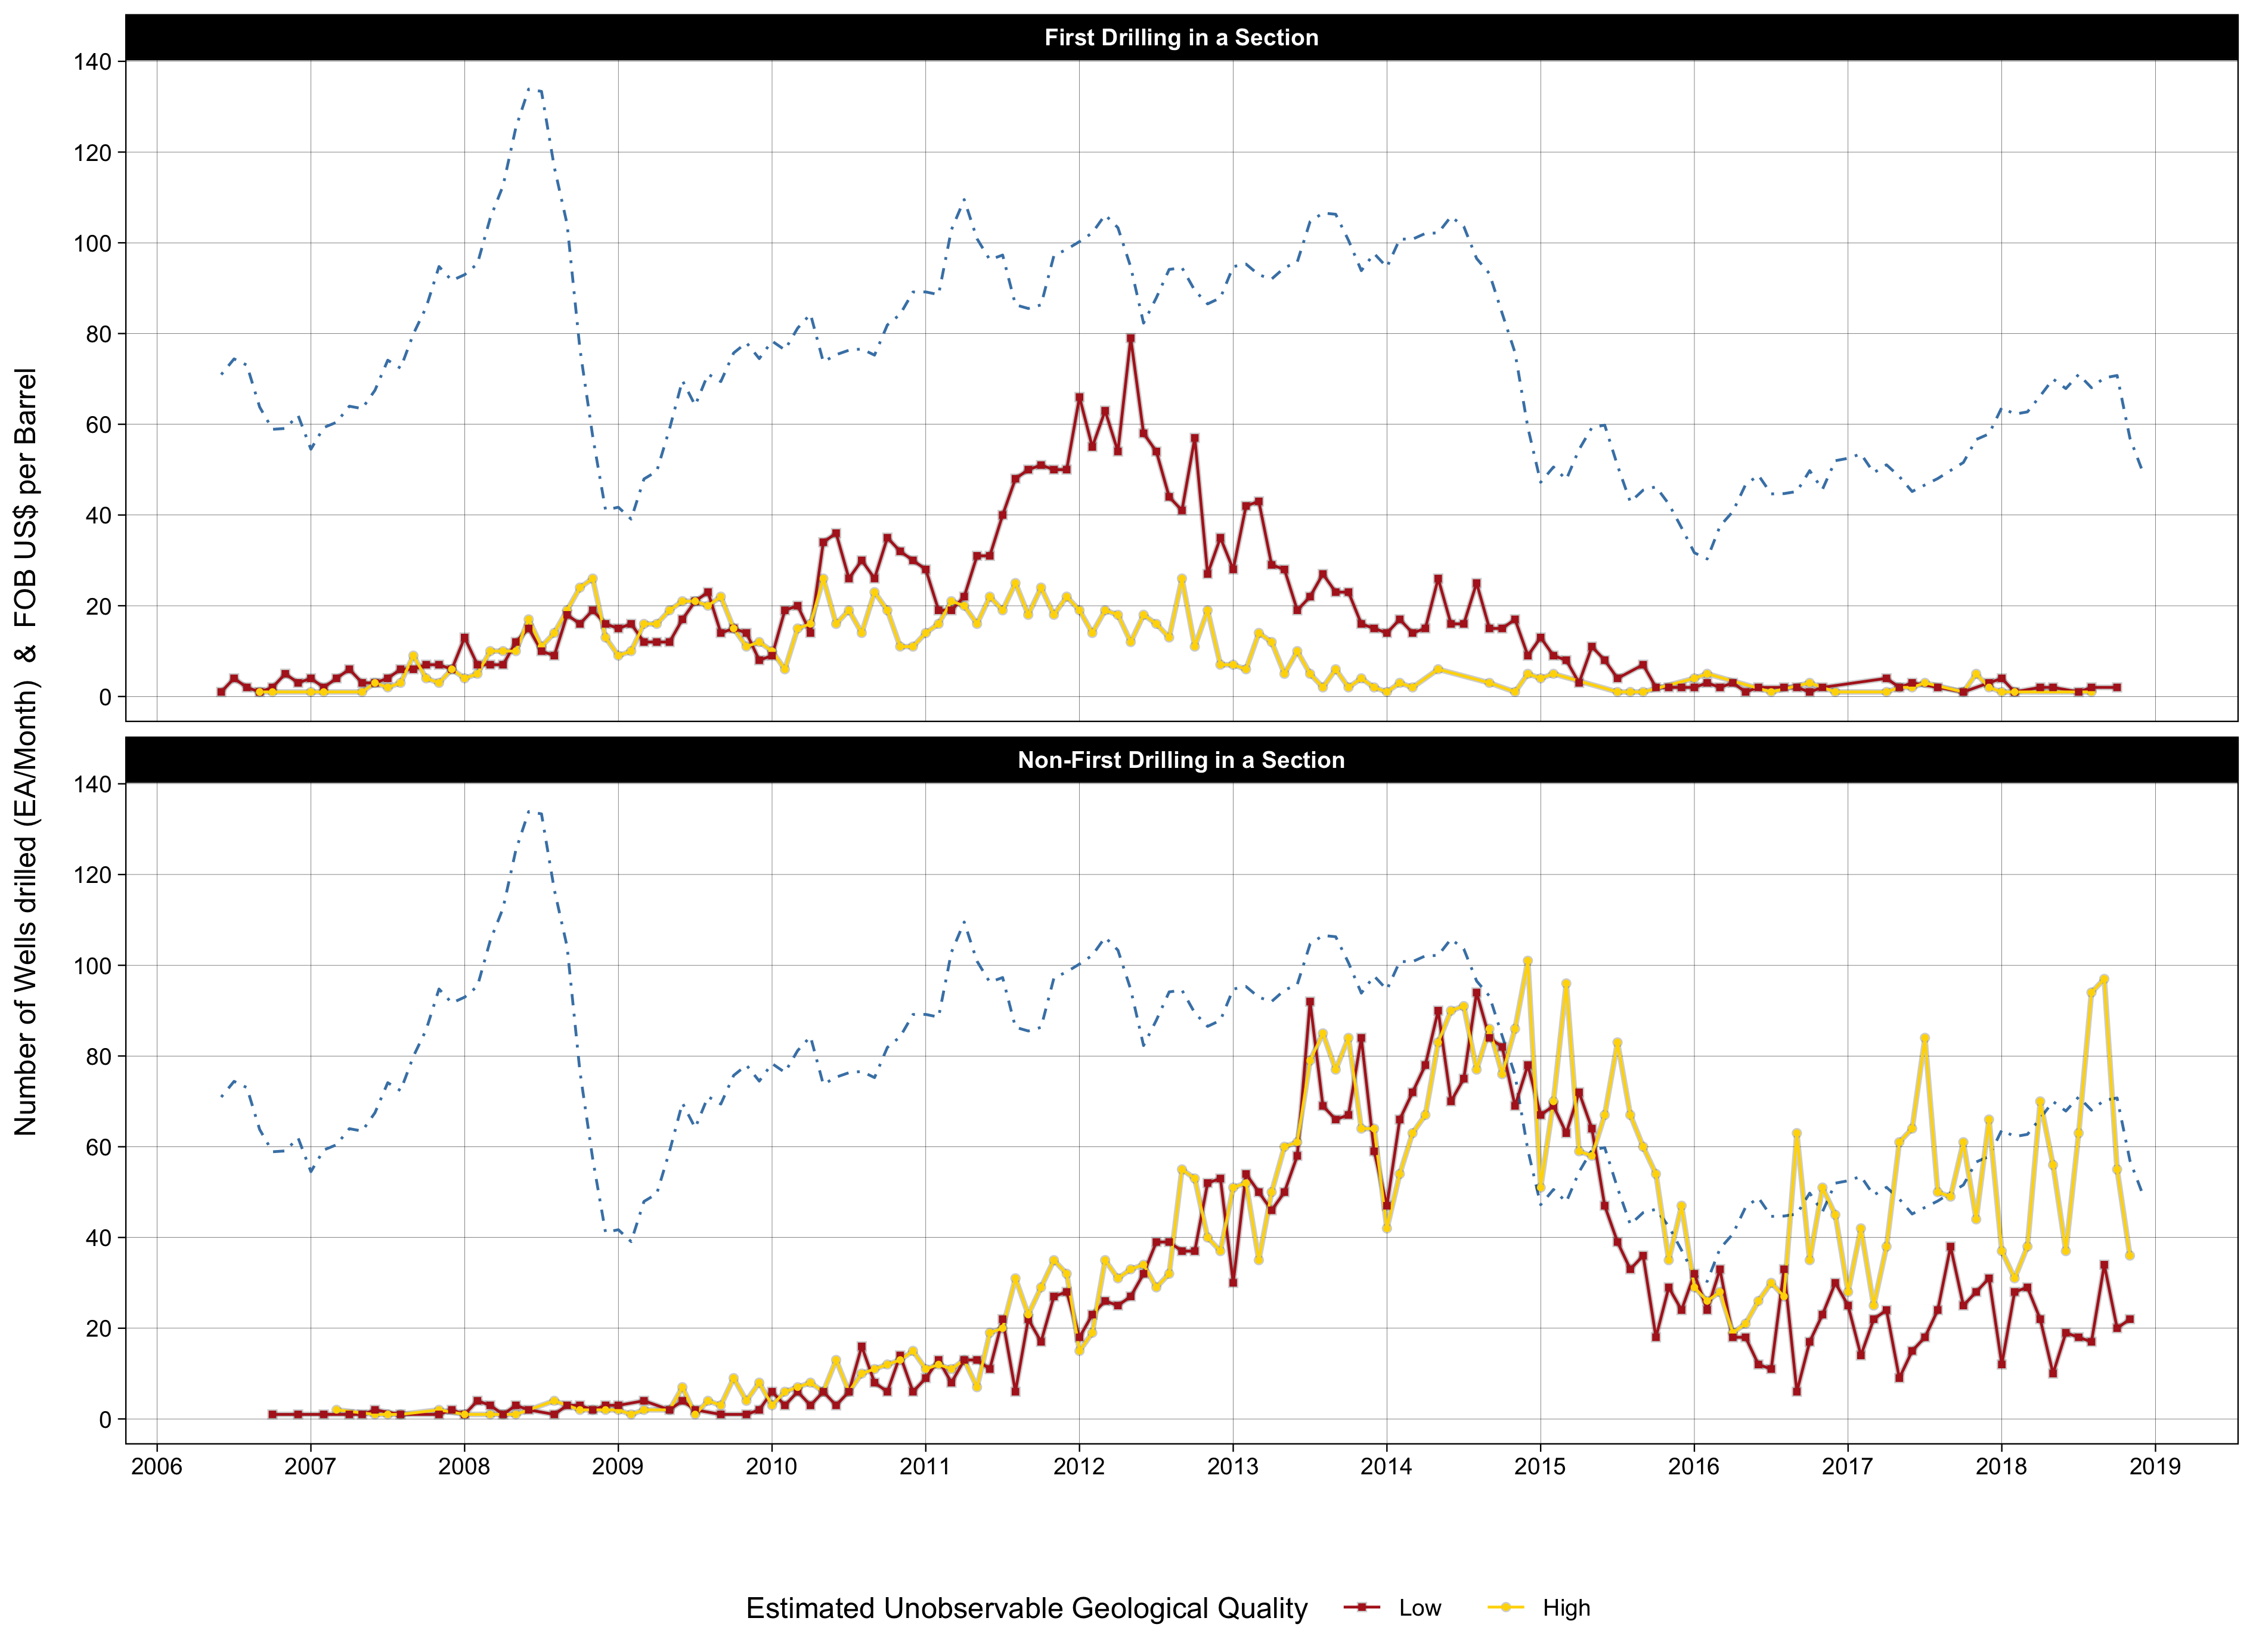
\includegraphics[scale = 0.12]{04_Chapter-3/00A_Figures/Figure_Drilling-over-Time_By-Well-Quality-and-Whether-First-Drilled.png}
        \caption{Held-by-Production vs. Non-Held-by-Production Horizontal Well Drilling}
        \caption*{
            {\small
            \textit{Note}: 
            This figure depicts the drilling of horizontal wells classified into two quality levels. The upper panel shows how the first drilling in each section, regarded as held-by-production drilling, has evolved. There was only a limited number of held-by-production drilling between 2015 and 2019. The lower panel indicates all subsequent drilling in sections. The collapse in oil prices between mid-2014 and 2015 made post-held-by-production drilling decrease. Drilling of low-quality well locations showed a more significant reduction, especially in 2015. High-quality sites were drilled more than low-quality ones during the period of oil price recovery from 2016 to 2019. In each panel, the dot-dashed line is the time series of the monthly per-barrel spot prices for West Texas Intermediate at Cushing, Oklahoma.
        }}
        \label{Figure:Held-by-Production-vs-Non-Held-by-Production-Horizontal-Well-Drilling}
    \end{figure}
}
Figure \ref{Figure:Held-by-Production-vs-Non-Held-by-Production-Horizontal-Well-Drilling} shows that drilling associated with held-by-production did not drive the relationship between oil prices and low-quality well drilling, especially between mid-2014 and the end of 2015. The upper panel in the figure illustrates the by-quality time series of the number of horizontal wells drilled that are supposed to be drilling related to Held-By-Production (HBP). In our empirical analysis, we assume that for each of the sections into which horizontal wells in our sample were drilled, the purpose of the first drilling in that section was just HBP.\footnote{In the Public Land Survey System, a \textit{section}, which is one of 36 sections in a township, is a one-mile-square area.} The relatively high drilling rate of low-quality wells, especially between mid-2011 and mid-2013, seems to be consistent with the empirical result of \cite{The-Economics-of-Time-Limited-Development-Options_2020_Herrnstadt-Kellogg-and-Lewis}: firms bound to a lease contract including use-it-or-lose-it requirements tend to drill low-productivity well locations just before the first lease expires.

The evolving pattern of drilling for each of the three quality levels presented in the lower panel of Figure \ref{Figure:Held-by-Production-vs-Non-Held-by-Production-Horizontal-Well-Drilling}, regarded as post-held-by-production drilling, shows completely different movements from those in the upper panel. Until 2014, horizontal wells of heterogeneous quality were drilled equally and at the same growth rate. But drilling of low-productivity horizontal wells more sensitively reacted to negative price shocks between mid-2014 and 2015, compared to drilling medium- and high-quality wells. The new theoretical approach, required to rationalize the simultaneous drilling of wells with heterogeneous qualities, needs to explain the high sensitivity of low-quality well drilling.